\documentclass{sty/eiiatfg}

% Hay muchos paquetes para LaTeX que facilitan centenares de trabajos
% engorrosos. Busca en Internet si no sabes hacer algo con LaTeX. El
% repositorio oficial está en https://ctan.org/

% Algunos paquetes especialmente útiles ya están incluídos en el estilo
% del TFG (consulta sty/eiiatfg.cls para más detalles).

% Cambia los datos de tu TFG aquí
% Si algun dato no quieres que figure borra la línea
\title{Usa \LaTeX{} para elaborar tu TFG}
\author{Francisco Moya Fernández}
\email{francisco.moya@uclm.es}
\director{Fernando Castillo García}
\tfgid{XX-A/B-XXXXXX}
\homepage{https://github.com/FranciscoMoya/eii-tfg}
\gitrepo{https://github.com/FranciscoMoya/eii-tfg}
\address{UCLM --- Escuela de Ingeniería Industrial\\
Campus Universitario de la Real Fábrica de Armas}
\zipcode{45071}
\phone{925 268 800 x.3729}

% Definición de acrónimos:
% \newacronym{id}{corto}{largo}

% Uso de acrónimos
% \acrshort{id} nombre corto
% \acrlong{id}  nombre largo
% \acrfull{id}  nombre largo (nombre corto)

\newacronym{TFG}{TFG}{Trabajo Fin de Grado}
\newacronym{CD}{CD}{Compact Disc}
\newacronym{GNU}{GNU}{GNU is Not Unix}
\newacronym{PDF}{PDF}{Portable Document Format}
\newacronym{TCPIP}{TCP/IP}{Pila de protocolos de Internet}
\newacronym{TCP}{TCP}{Transport Control Protocol}
\newacronym{XML}{XML}{eXtensible Markup Language}


% La bibliografía la puedes descomponer en varios archivos .bib
% Los archivos .bib se pueden escribir a mano con ayuda de un editor online
% (e.g. http://truben.no/latex/bibtex) o generar con Mendeley u otro
% gestor de bibliografía. Solo se incluyen las referencias que son citadas
% en el texto.
\addbibresource{bib/main.bib}
\addbibresource{bib/how.bib}
\addbibresource{bib/ejemplos.bib}

\begin{document}

% Puedes cambiar la licencia de este documento con la orden license.  Por defecto se asume Creative Commons Attribution 4.0 (ver https://creativecommons.org/licenses/by/4.0/).  
% Por ejemplo, para restringir su uso, copia y distribución:
%\license{Todos los derechos reservados.}

% Si usas muchos símbolos conviene que describas lo que significan en un archivo
% aparte (en este caso simbolos.tex).  Si no es el caso puedes comentar esta línea
\listofsymbols{simbolos.tex}

\portada

% Edita los
\begin{agradecimientos}
Pon aquí tus agradecimientos, pero no te olvides de que se trata de un documento profesional.
\end{agradecimientos}	   
\begin{dedicatoria}
Aquí va la dedicatoria.
\end{dedicatoria}
\begin{resumen}

\avisoLocalizacionArchivo

\noindent Aquí va el resumen en español. Debería ocupar entre 1000 y 1500 palabras a modo orientativo.

\warning{Escribe el resumen en estilo periodístico, desde lo más general a lo más específico.  Desde lo más importante a lo menos importante.  Esto será especialmente útil si es necesario hacer un resumen más breve en otro contexto (presentación, herramienta, etc).  Si el resumen está en formato periodístico bastará con seleccionar los primeros párrafos.}
\end{resumen}

\begin{abstract}
\noindent  Write down the abstract in English here. It must be between 1000 and 1500 words long.
\end{abstract}


\indices

% El cuerpo del documento está en la carpeta tex
% Aquí simplemente se incluyen los archivos correspondientes a cada capítulo.

% No los llames capitulo1, capitulo2, etc. Los números los pondrá LaTeX según
% el orden en que los pongas.  Eso facilitará después su posible reordenación
% o división.

% Esta estructura corresponde a un documento científico-técnico.
% Si ves que tu proyecto concuerda con un trabajo profesional organiza el 
% documento según UNE 157001

\chapter{Introducción} 
\label{ch:introduccion}

En este capítulo debes introducir el problema sin divagar, sin copiar de otros documentos y sin utilizar un lenguaje excesivamente técnico.  Tampoco utilices un lenguaje informal.  Este capítulo debería convencer al cliente de que el proyecto merece la pena.  Es decir, es un problema real y no está resuelto completamente.

Debe tenerse siempre presente que el cliente es el que paga.  En el TFG el que paga es el tribunal, en forma de calificación.  Así que a quien hay que convencer es a los miembros del tribunal.  El tribunal no lo conocerás a priori.  Por eso la memoria debe estar escrita para que la entienda alguien que no es especialista en el campo de aplicación.  Pero eso no implica que se toleren la falta de rigor o la falta de argumentación técnica.  Solo implica que los argumentos específicos hay que explicarlos o citar la fuente que los explica.

Redacta la introducción al final del TFG, cuando tengas elaborado el capítulo de antecedentes, los resultados y su discusión.  De esta forma podrás evitar repetir argumentos que ya están en esos capítulos.  La introducción debe introducir también el contexto en el que se desarrolla el TFG.  Divide el documento en secciones y subsecciones para organizar el contenido del capítulo.  Utiliza preferentemente frases cortas.


\section{Organización de la memoria} 
\label{sec:organizacion-memoria}

La organización de este documento responde a un documento científico-técnico. Se descompone en los siguientes capítulos.

\begin{description}
    \item[\autoref{ch:objetivos}] Enumera y justifica los objetivos del proyecto y establece los límites intrínsecos y extrínsecos de ejecución del TFG.
    \item[\autoref{ch:antecedentes}] Analiza los antecedentes y estado del arte en relación al tema del proyecto.
    \item[\autoref{ch:desarrollo}] Describe todo el proceso de desarrollo del TFG.  Esto incluye la metodología de trabajo empleada y las diferentes etapas o iteraciones que se han llevado a cabo.  No dudes en descomponer el capítulo en varios si aglutina demasiado material.
    \item[\autoref{ch:resultados}] Describe en detalle los resultados obtenidos y las pruebas realizadas. Discute los resultados en relación a los objetivos del proyecto.
    \item[\autoref{ch:conclusiones}] Recopila las principales conclusiones del proyecto y comenta las líneas de trabajo futuro, en caso de que se contemplen.
    \item[\deschyperlink{ch:anexos}{Anexos}] Complementan la información del cuerpo del documento con información técnica útil para reproducir los resultados, pero innecesaria para comprender en su totalidad el TFG realizado.
    \item[\deschyperlink{ch:bibliografia}{Bibliografía}] Recopila las referencias bibliográficas utilizadas en este documento.
\end{description}

\warning{Al finalizar el resto de los capítulos revisa esta descripción del documento para que coincida con lo que realmente contiene la memoria.  Por ejemplo, es frecuente fusionar varios capítulos en uno cuando son muy pequeños.  También es frecuente lo contrario, dividir un capítulo en varios cuando es muy extenso.}

\section{Repositorio de información}
\label{sec:repositorio}

\warning{Es muy útil tanto para la ejecución como para la evaluación disponer de un repositorio para almacenar las sucesivas versiones del documento y de todo el material generado durante el proyecto.  La UCLM está gestionando la incorporación de \href{https://github.com}{GitHub} como servicio institucional.  Otras posibilidades son \href{https://gitlab.com}{GitLab} o \href{https://bitbucket.org}{BitBucket}. Si no utilizas un repositorio quita esta sección.}

Todo el material generado durante la ejecución de este proyecto está disponible en el repositorio \thegitrepo{}.  El material incluye el código \LaTeX{} del presente documento, el código fuente de los programas realizados o modificados, y todos los datos generados en la evaluación de resultados.
\chapter{Objetivos}
\label{ch:objetivos}

Primero enumera los objetivos, no los resumas ni los redactes en un párrafo.  Cada uno de los objetivos de un proyecto debe ser SMART:

\begin{description}
\item[Simple] Cada objetivo tiene que ser independiente, tener sentido por sí mismo y más o menos indivisible.  Si no es suficientemente indivisible, pero tiene sentido como una entidad independiente, debes descomponerlo en subobjetivos.
\item[Medible] Tiene que ser posible medir el grado de consecución al final del TFG.
\item[Acordado] Los objetivos no los pones tú solo.  Deben partir de un acuerdo con tu director.
\item[Realista] No pongas objetivos muy ambiciosos. Basta con que resuelva el problema de la forma más simple posible.  Si superas los objetivos nadie se va a quejar.  El director se encargará de que tampoco sean demasiado poco ambiciosos.
\item[Temporizado] Un objetivo debe tener un marco temporal. Si no es así el objetivo podría no cumplirse nunca.  Es difícil poner límites temporales muy estrictos en un primer proyecto de ingeniería, pero al menos acota.
\end{description}

Tras cada objetivo puedes añadir párrafos ampliando la descripción del objetivo, describiendo los límites y justificándolos.  También puedes describir de qué se parte.  Si es posible debería quedar plenamente justificado que se trata de objetivos SMART.  Considera tanto límites intrínsecos (inherentes a la definición del proyecto) como extrínsecos (limitaciones presupuestarias, equipamiento disponible, etc).
\chapter{Motivación y antecedentes}
\label{ch:antecedentes}

El problema que pretendes resolver está dentro de un contexto que el cliente debe conocer.  Esta sección aporta información para conocer en detalle la importancia del problema y la dificultad para resolverlo con los productos y programas disponibles actualmente.

Este capítulo concentrará el grueso de las citas del TFG.  Dado que se trata del primer trabajo profesional, el alumno no suele estar familiarizado con las citas bibliográficas.  Pon toda tu atención en qué citas y cómo lo citas.  Revisa la sección~\ref{sec:bibliografia-citas} para las reglas mínimas que deben cumplir las citas.

\warning{Es muy importante respetar la regla de atribuir correctamente.  No es aceptable desde el punto de vista legal, ni tampoco desde el punto de vista ético, copiar trabajo de otros sin atribuirlo correctamente a los autores.}

Esta sección debe estudiar de forma sistemática todas las opciones ya disponibles en la actualidad para resolver el problema. No basta con una mera enumeración, hay que estudiarlos mínimamente para explicar por qué no son una solución para el problema o qué podría aportar a la solución del problema.

Un método sistemático para realizar esta parte del TFG es la revisión sistemática de literatura, conocida habitualmente por sus siglas en inglés SLR (\emph{Sistematic Literature Review}).  Un resumen muy sencillo de cómo realizar una SLR puede encontrarse en~\cite{anderskofodpetersen2014}.  También encontrarás consejos prácticos en~\cite{sandroschulze2017}.  Para un proceso más detallado, especialmente si tu problema tiene mucho arte previo, puedes consultar~\cite{barbarakitchenhamstuartcharters2007}.  Si no hay mucho arte previo pon este capítulo y el siguiente juntos.

En una tesis doctoral el análisis sistemático del estado del arte es esencial. En un TFG es importante, pero no hay que perder la cabeza.  Un TFG son unas 300 horas de trabajo de un estudiante medio que ya posea los conocimientos generales necesarios (volveremos a esto más tarde).  Considero que un buen análisis del estado del arte corresponde a un trabajo de entre 25 horas y 100 horas, dependiendo del tema del proyecto.  Si el tema es muy específico es más fácil hacer el estudio del estado del arte.

Termina este capítulo con una sección que resuma el estado del arte e identifique las lagunas lo más claramente posible.  Una tabla comparativa o un gráfico pueden ser formas interesantes de presentar la información.
\chapter{Desarrollo del TFG}
\label{ch:desarrollo}

\avisoLocalizacionArchivo 

En general este capítulo debe describir cómo se ha llegado a la solución del problema incluyendo metodología, planificación y ejecución.

En primer lugar, este capítulo debe tratar con la metodología de trabajo empleada para elaborar el TFG.  La metodología puede variar sustancialmente dependiendo del contexto o el área temática en la que se encuadre.  Si es necesario, divide la descripción de la metodología como capítulo independiente.

A continuación, debe describir cómo se ha dividido el problema en una secuencia de fases, tareas o iteraciones y qué cantidad de recursos (tiempo fundamentalmente) se han planificado para cada una.

Por último, debe incluir información sobre la ejecución del proyecto. Cuáles han sido los problemas encontrados y qué desviaciones se han producido en la ejecución.  Dependiendo de la naturaleza del proyecto es posible organizar esta información de manera conjunta con la planificación.

\chapter{Resultados y discusión}
\label{ch:resultados}

\avisoLocalizacionArchivo 

Escribe en este capítulo los resultados del proyecto.  Este capítulo debería explicar los resultados de forma global, no los resultados de cada fase o iteración.  Probablemente será el capítulo con más tablas y gráficas.  Revisa las secciones~\ref{sec:figuras} y~\ref{sec:tablas} para aprender cómo se escriben en \LaTeX{}.

Tus contribuciones no tienen por qué limitarse al trabajo sistemático del TFG.  Puede que hayas contribuido en aspectos metodológicos, en ideas novedosas, en la planificación de experimentos, en desarrollos matemáticos. Este capítulo está para agrupar todo eso.  Describe con claridad todo lo que ha supuesto contribuciones originales por tu parte.

\warning{Es importante destacar que un resultado negativo es también un resultado.  Es posible que el proyecto planteara abordar un problema con un método que ha demostrado ser no apto.  Si el trabajo ha sido sistemático sigue teniendo mucho valor, puesto que excluye el método para cualquier otro trabajo futuro.  Escribe este tipo de resultados con especial cuidado para destacar que el trabajo se ha realizado de manera sistemática.}
\chapter{Conclusiones}
\label{ch:conclusiones}

Las conclusiones deben cerrar el documento, destacando los aspectos más importantes de la ejecución del TFG.  Debe analizar qué objetivos se han alcanzado y en qué grado, qué objetivos se han tenido que dejar fuera del proyecto y por qué, y qué líneas de trabajo futuro abre el TFG. 

Fíjate en que los objetivos abren el trabajo personal y las conclusiones lo cierran.  Procura mantener un orden que resalte esta relación, pero no te limites a parafrasear los objetivos.

% Los anexos pueden ir en la misma carpeta que el cuerpo del documento 
% porque eso facilita la migración de partes de un capítulo a un anexo.
\appendix\cleardoublepage
\hypertarget{ch:anexos}{%
    \chapter{Chuleta de \LaTeX{}}
\label{ch:latex}

\LaTeX{} es un formato textual para construir documentos complejos, cualquier tipo de documento complejo.  No es difícil, y de hecho está pensado para que personas sin formación en tipografía y composición puedan redactar documentos estéticamente impecables.  Pero necesita algo de tiempo para acostumbrarse a la filosofía.

Puedes acabar tu TFG simplemente imitando la redacción de este documento, pero seguro que puedes sacar más partido si aprendes algo de \LaTeX{}.  Hay muchas guías sencillas para empezar. Por ejemplo,~\cite{ernestoaranda2013} o~\cite{gastonsimone2002} son resúmenes suficientemente completos y sencillos.  En caso de que quieras ampliar tus conocimientos tendrás que empezar por el libro de Leslie Lamport~\cite{leslielamport1994}, el creador de \LaTeX{}.  Procura complementarlo con~\cite{latexcompanion2004} y, especialmente, navegar por el \href{https://ctan.org}{CTAN} (\emph{Comprehensive \TeX{} Archive Network}).  CTAN es un repositorio enorme de paquetes, que facilitan la edición de todo tipo de detalles.  Desde las cabeceras de página, hasta la creación de enlaces hipertexto o el manejo de colores.

En este anexo se incluye un pequeño recetario, extraído de la plantilla de Fernando Castillo, que puedes usar a modo de recordatorio rápido, pero procura utilizar una referencia más completa cuando empieces a editar el documento.

\warning{Este recetario no es un libro de \LaTeX{}, ni es para sentarse a leerlo, es para usarlo cuando lo necesites.  No te mostramos cómo se escribe en \LaTeX{} cada ejemplo, sino que directamente lo hacemos.  Cuando necesites hacer algo semejante, mira el código de este documento en \url{https://github.com/UCLM-eiia-to/eiia_doc_tfg_latex}}

\section{Texto} 
\label{sec:texto}

\noindent En esta sección se muestran ejemplos de efectos de texto.

\begin{description}
\item[\texttt{textbf}] \textbf{Texto en negrita.}

\item[\texttt{textit}] \textit{Texto en cursiva.}

\item[\texttt{underline}] \underline{Texto subrayado.}

\item[\texttt{large}] {\large Texto grande}

\item[\texttt{Large}] {\Large Texto más grande}

\item[\texttt{LARGE}] {\LARGE Texto mucho más grande}

\item[\texttt{textsc}] \textsc{Texto en versalitas}

\item[\texttt{textsf}] \textsf{Texto en fuente sans-serif}

\item[\texttt{texttt}] \texttt{Texto en fuente mono-espaciada}
\end{description}

A veces resulta útil este tipo de texto para funciones de programación o código fuente. Por ejemplo:

\begin{verbatim}
    [x,y]=function(t,z) 
\end{verbatim}

\subsection{Listas numeradas y con viñetas} 

Listas numeradas. Se utilizan cuando la posición que ocupan los elementos es importante, para contar los elementos, o cuando se necesita añadir referencias a algunos de los elementos.

\begin{enumerate}
\item diodos
\item transistores
    \begin{enumerate}
    \item transistores pnp
    \item transistores npn
    \item operacionales
    \end{enumerate}
\item operacionales
\end{enumerate}

Listas con viñetas. Se utilizan cuando la posición concreta de los elementos no es importante:

\begin{itemize}
\item diodos
\item transistores
    \begin{itemize}
    \item transistores pnp
    \item transistores npn
    \item operacionales
    \end{itemize}
\item operacionales
\end{itemize}

\subsection{Acrónimos}

Si quieres lista de acrónimos debes marcar los acrónimos con una etiqueta especial.  Por ejemplo, así se pondría la primera vez un \acrfull{CD}.  Una vez que se ha usado el acrónimo, ya se puede usar en forma abreviada, como en~\acrshort{CD}.  Marca incluso en este caso los acrónimos, porque así el PDF permitirá navegar a la definición pinchando sobre él.

\section{Figuras}
\label{sec:figuras}

En esta sección se muestran algunos ejemplos de figuras.  Utilizaremos algo de texto de relleno para ver cómo coloca \LaTeX{} las figuras.

La fig.~\ref{fig:figurita-ejemplo} es un ejemplo de \emph{Encapsulated PostScript}.  Se trata de un formato vectorial, que no se degrada al escalarlo.  Este tipo de formatos son los ideales para usar con \LaTeX{}.  Utiliza siempre que puedas imágenes en formato EPS o PDF.

\begin{figure}[hbtp]
\centering
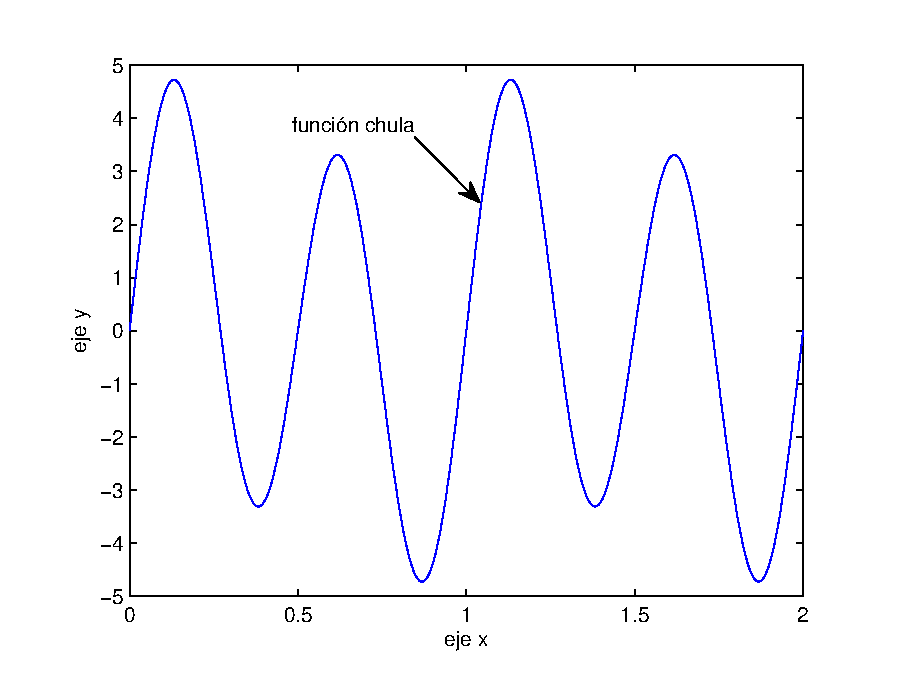
\includegraphics[scale=0.5]{ejemplo.eps}
\caption{Figurita ejemplo}
\label{fig:figurita-ejemplo}
\end{figure}

La forma de incluir la figura es simple:

\begin{minted}{latex}
\begin{figure}
\centering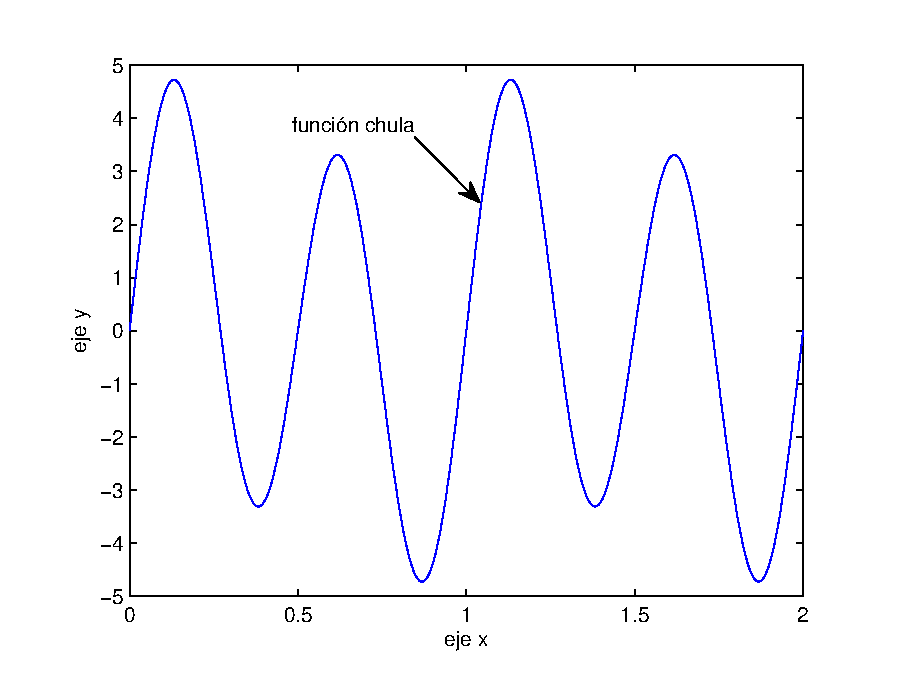
\includegraphics[width=6cm]{ejemplo.eps}
\caption{Figurita ejemplo}
\label{fig:figurita-ejemplo}
\end{figure}
\end{minted}

El entorno \texttt{figure} crea un cuadro flotante, con todo el contenido de la figura, que \LaTeX{} coloca en el sitio menos malo.  La \texttt{caption} es el pie de la figura y la \texttt{label} es la etiqueta que nos permitirá referirnos a ella en el texto (con la orden \texttt{ref}).

\LaTeX{} utiliza un algoritmo nada evidente para colocar las figuras de manera que sea estéticamente agradable.  Pero tú puedes influir en las preferencias de colocación.  El entorno \texttt{figure} tiene un parámetro opcional entre corchetes que indica las opciones de colocación.  Por defecto es \texttt{[tbp]}, que equivale a \emph{top, bottom, page}.  Eso quiere decir que intenta primero ponerla a comienzo de página.  Si no lo consigue, al final de una página.  Y si así tampoco lo consigue, en una página entera, solo para la figura.  En este ejemplo utilizo las opciones \texttt{[hbtp]} para que intente la secuencia \emph{here, bottom, top, page}.  En este caso prefiero que la ponga debajo antes que arriba, para que no aparezca en una sección anterior.

Con \LaTeX{} puedes conseguir que las figuras no se muevan en absoluto, pero eso deja documentos extremadamente descompensados.  No lo hagas nunca.  Es mejor mover ligeramente la figura en el texto o incluso re-escribir parte del texto, antes de forzar la posición.  De todas formas, si no me quieres hacer caso, en la fig.~\ref{fig:figurita-ejemplo-2}  tienes un ejemplo que fuerza la posición.

\begin{figure}[h!]
\centering
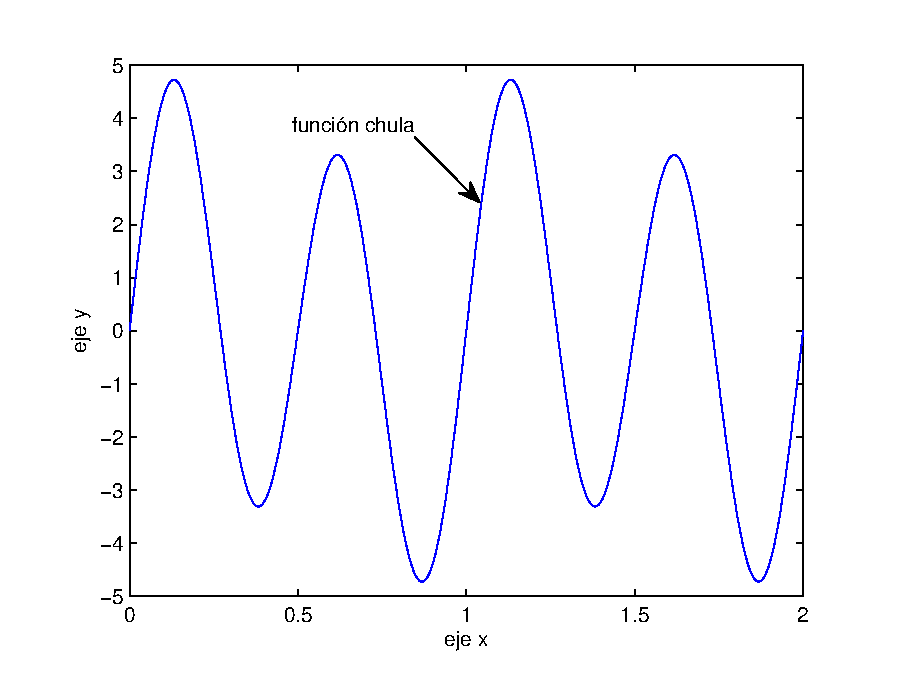
\includegraphics[scale=0.5, angle=15]{ejemplo.eps}
\caption{Figurita ejemplo 2}
\label{fig:figurita-ejemplo-2}
\end{figure}

Para poder poner figuras que no son de elaboración propia es necesario primero obtener permiso del autor y, además, añadir la fuente al pie de foto. Hay muchas guías de estilo que explican en detalle cómo hacerlo. Por ejemplo, la \emph{American Psychological Association} tiene un \href{https://www.lib.sfu.ca/help/research-assistance/format-type/online-images/citing#citing-images-in-apa}{capítulo específico de su manual de publicaciones}.  El manual de la APA se usa extensivamente en todo tipo de literatura científica.

\begin{figure}[htb]
\centering
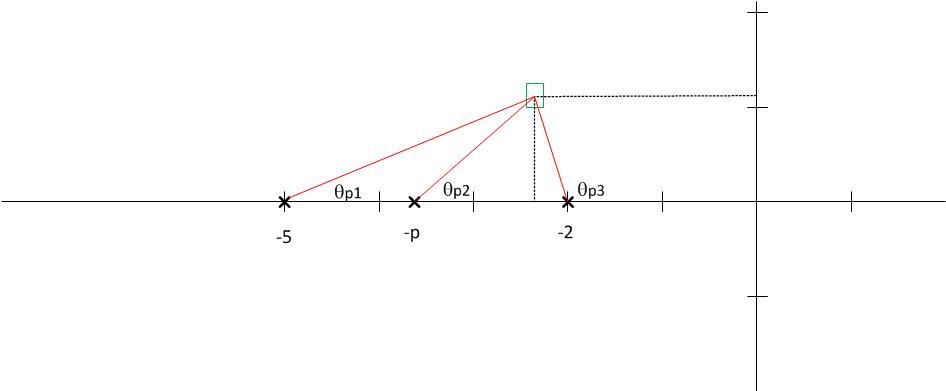
\includegraphics[scale = 0.5]{ejemplo2.jpg}
\caption{Figurita ejemplo 3. Extraída de la plantilla de TFG de Fernando Castillo. \copyright 2018 Fernando Castillo. Reproducida con permiso.}
\label{fig:figura-ejemplo-3}
\end{figure}

\warning{Fíjate bien.  No se citan las imágenes como si se tratara de referencias bibliográficas.  No debe haber pie de página (orden \texttt{footnote}) ni cita (orden \texttt{cite}) en un pie de foto (\texttt{caption}).  La atribución de la obra debe estar al mismo nivel que la obra usada.  Por eso debe atribuirse completamente en el pie de foto.}

Se puede controlar el escalado de la imagen y el ángulo de forma muy sencilla, con las opciones de la orden \texttt{includegraphics}.  En la fig.~\ref{fig:figura-ejemplo-3} se muestra un ejemplo de figura escalado a un 30\%.  La orden \texttt{includegraphics} ajusta los parámetros de la imagen para mantener la relación de aspecto original, si esto es posible.  Esto hace que podamos especificar simplemente el ancho o el alto deseado, que va a ser lo más habitual.  En mi opinión, las opciones más frecuentes de \texttt{includegraphics} son, por orden:

\begin{figure}
\centering
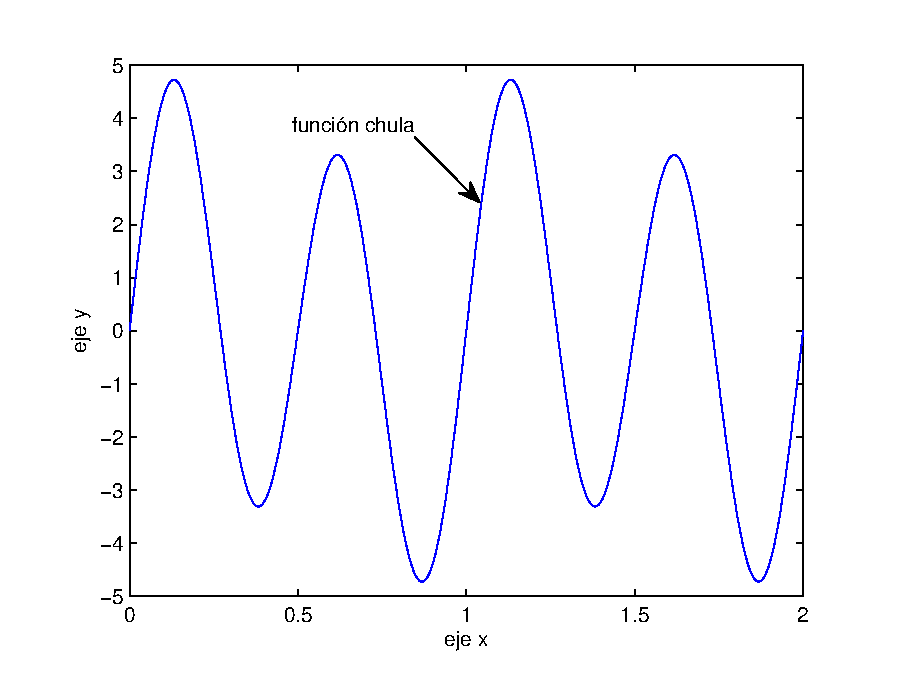
\includegraphics[width=\textwidth]{ejemplo.eps}
\caption{Figura ejemplo que ocupa todo el ancho del texto.}
\label{fig:figura-ejemplo-4}
\end{figure}

\begin{description}
\item[\texttt{width}]  Fija el ancho de la imagen.  Puede ser un tamaño absoluto en centímetros (\texttt{cm}), milímetros (\texttt{mm}) o puntos PostScript (\texttt{pt}).  Por ejemplo,  \verb|width=1.5cm|.  También puede ser un tamaño relativo a cualquier medida del documento.  Por ejemplo, \verb|width=0.5\textwidth| sería una figura que ocupe la mitad del ancho del texto.

\item[\texttt{height}] Fija la altura de la imagen.  Es similar a \texttt{width} pero con la altura.  Se puede especificar tanto altura como anchura, de manera que se modifica la relación de aspecto original.

\item[\texttt{scale}] Utiliza un factor de escala para la imagen.  Puede ser mayor de 1 para ampliar la imagen.

\item[\texttt{angle}] Gira la imagen un número de grados determinado.  Si el número es negativo el giro es en sentido horario.  Si es positivo el giro es antihorario.
\end{description}


En la fig.~\ref{fig:figura-angulo-30} se muestra un ejemplo de figura girada 30.

\begin{figure}[btp]
\centering
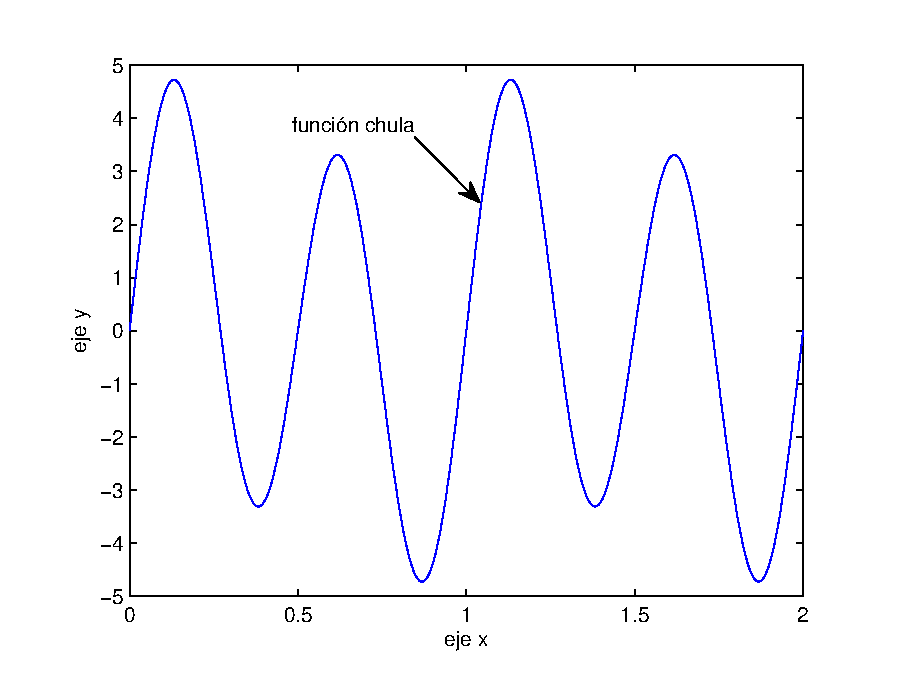
\includegraphics[width=.3\textwidth,angle=-30]{ejemplo.eps}
\caption{Figura ejemplo de rotación.}
\label{fig:figura-angulo-30}
\end{figure}

Una característica interesante del entorno \texttt{figure} es que permite definir sub-figuras con la orden \texttt{subfigure} o el entorno del mismo nombre.  La colocación de las sub-figuras es prácticamente automática.  Un ejemplo puede verse en la figura~\ref{fig:matriz-figuras}.

\begin{figure}[htbp]
\centering
\subfigure[figurita1]{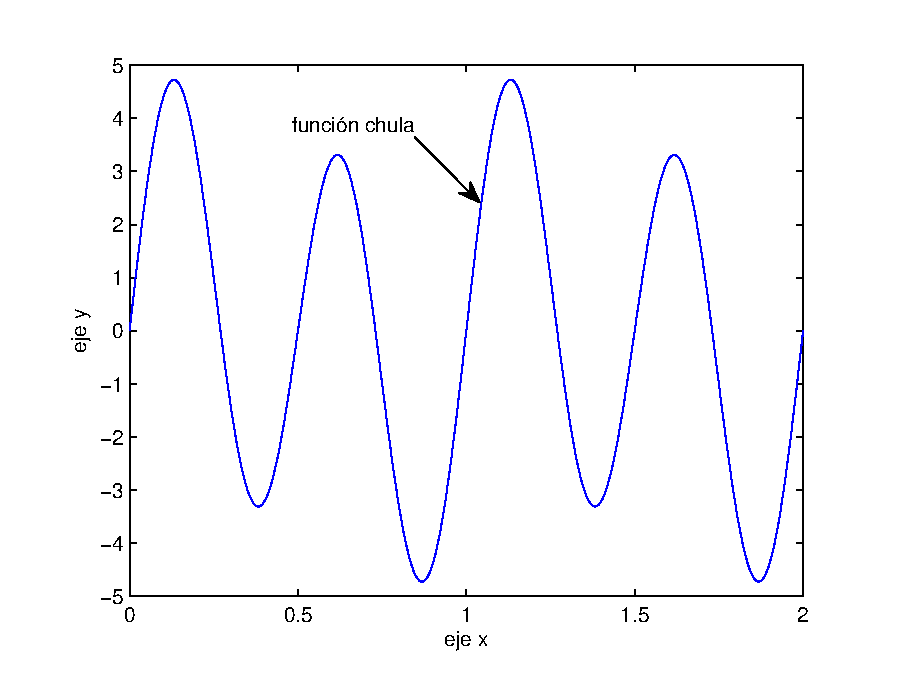
\includegraphics[width=40mm]{ejemplo.eps}}
\subfigure[figurita2]{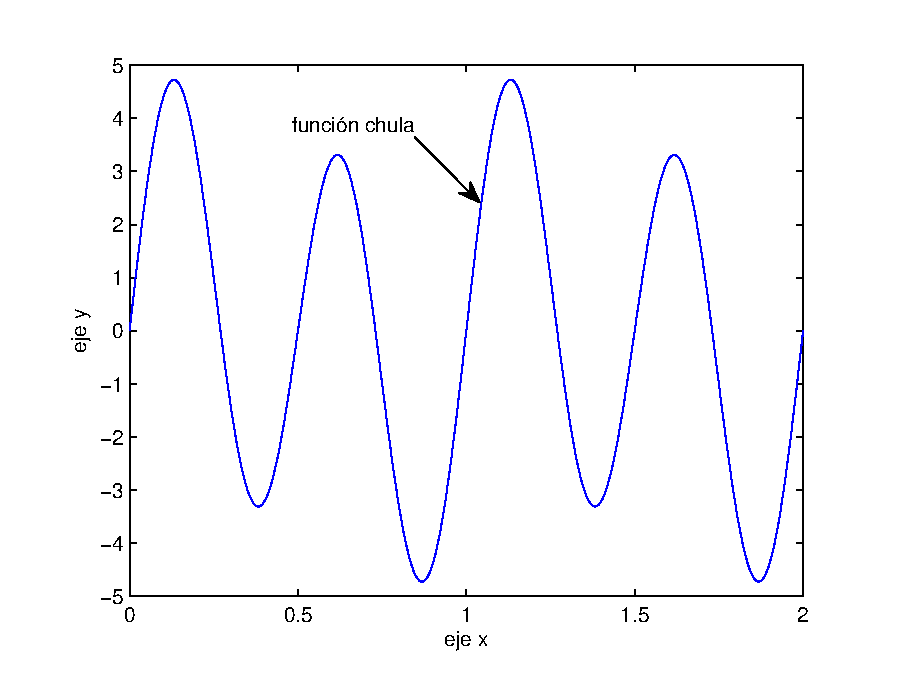
\includegraphics[width=40mm]{ejemplo.eps}}
\subfigure[figurita3]{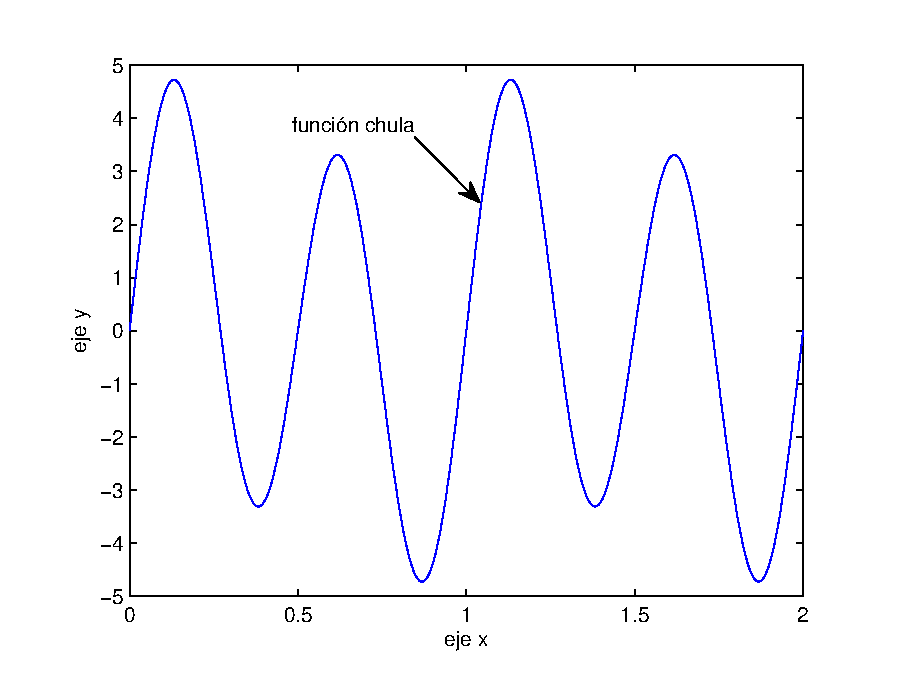
\includegraphics[width=80mm]{ejemplo.eps}}
\caption{Matriz de figuras} 
\label{fig:matriz-figuras}
\end{figure}

Una subfigura puede referenciarse a partir de la referencia a la figura.  Por ejemplo, la figura~\ref{fig:matriz-figuras}(a) es igual que la figura~\ref{fig:matriz-figuras}(b). Sin embargo, cuando las figuras son muy complejas, es posible que se prefieran esquemas más automáticos.  En \href{https://tex.stackexchange.com/questions/181225/how-to-reference-to-subfigure-in-latex}{StackExchange} encontrarás soluciones a éste y otros problemas con mucha facilidad.

En general, he tratado de mantener un compromiso entre el número de características incluidas y la facilidad de uso de la plantilla.  Las figuras muy complejas es algo que prefiero evitar, así que en el estilo de la plantilla no incorpora los paquetes \texttt{subcaption} y \texttt{cleveref}.

\section{Tablas} 
\label{sec:tablas}

En esta sección se muestran algunos ejemplos de tablas.

\begin{table}[htb]
\centering
\vspace{2mm}
\begin{tabular}{|c|c|c|}
\hline
 Regulador & Función de Transferencia & orden  \\
 \hline
 P         & $\alpha_1$               & 2      \\
 \hline
\end{tabular}
\caption{Resultados de la simulación}
\label{tab:resultados-simulacion}
\end{table}

Las tablas en \LaTeX{} no son complejas pero puedes simplificar aún más usando un editor interactivo de tablas.  Por ejemplo, en \url{https://truben.no/table/} hay una aplicación \emph{online} para editar multitud de formatos de tablas.  Es especialmente útil para tablas complicadas.

En \LaTeX{} es bastante frecuente separar la cabecera del cuerpo de la tabla poniendo dos \texttt{hline}, como en la tabla~\ref{tab:sencilla}.

\begin{table}[htb]
\begin{center}
\begin{tabular}{|l|l|}
\hline
País     &    Ciudad \\ \hline \hline
España   &    Madrid \\ \hline
España   &    Valencia \\ \hline
Francia  &    París \\ \hline
\end{tabular}
\caption{Tabla muy sencilla.}
\label{tab:sencilla}
\end{center}
\end{table}

La complejidad empieza cuando hay que expandir celdas para ocupar varias columnas o varias filas.  Por ejemplo, la tabla (\ref{tab:dificililla}) tiene una celda multi-columna y otra celda multi-fila.  En estos casos un editor interactivo como el de \href{https://truben.no/table/}{Peder Lång Skeidsvoll} puede ser de gran ayuda para un principiante.  Explora las opciones, no son evidentes al principio.

\begin{table}[htb] 
\centering
\begin{tabular}{|c|c|}
\hline
\multicolumn{2}{|c|}{Europa} \\
\hline
País  & Ciudad \\ \hline \hline
\multirow{2}{1.1cm}{España} & Madrid \\ \cline{2-2}
& Valencia \\ \hline
Francia & París \\ \hline
\end{tabular}
\caption{Fusionando celdas.}
\label{tab:dificililla}
\end{table}

Las tablas, al igual que las figuras, tienen un parámetro opcional entre corchetes que indican las preferencias de posición.  Se puede forzar pero, al igual que con las figuras, conduce a documentos muy descompensados.  Procura evitarlo.  Dentro de la tabla se define un entorno \texttt{tabular} que indica con su argumento obligatorio las columnas.  Este entorno es muy útil en cualquier organización matricial.  Se puede usar también para presentar las subfiguras de una figura, o para definir una matriz.

Las tablas muy largas deben dividirse en varias páginas.  En el estilo de este TFG hemos incluído el paquete \texttt{longtable}, que facilita enormemente escribir este tipo de tablas largas.  En ese caso, en lugar del entorno \texttt{table} y el entorno \texttt{tabular} se usaría solamente el entorno \texttt{longtable}, que es una especie de híbrido de los dos, con un montón de características opcionales.  Para ilustrar su uso reproducimos \href{https://texblog.org/2011/05/15/multi-page-tables-using-longtable/}{un ejemplo de TeXblog} en la tabla~\ref{tab:tabla-larga}.

\begin{center}
\begin{longtable}{|c|c|c|c|}
\caption{Un ejemplo de tabla larga}
\label{tab:tabla-larga}\\
\hline
\textbf{Primera} & \textbf{Segunda} & \textbf{Tercera} & \textbf{Cuarta} \\
\hline
\endfirsthead
\multicolumn{4}{c}%
{\scriptsize\textbf{\tablename\ \thetable}\ -- \textit{Continúa de la página anterior}} \\
\hline
\textbf{Primera} & \textbf{Segunda} & \textbf{Tercera} & \textbf{Cuarta} \\
\hline
\endhead
\hline \multicolumn{4}{r}{\textit{\scriptsize Continúa en la página siguiente}} \\
\endfoot
\hline
\endlastfoot
1 & 2 & 3 & 4 \\ 1 & 2 & 3 & 4 \\ 1 & 2 & 3 & 4 \\ 1 & 2 & 3 & 4 \\
1 & 2 & 3 & 4 \\ 1 & 2 & 3 & 4 \\ 1 & 2 & 3 & 4 \\ 1 & 2 & 3 & 4 \\
1 & 2 & 3 & 4 \\ 1 & 2 & 3 & 4 \\ 1 & 2 & 3 & 4 \\ 1 & 2 & 3 & 4 \\
1 & 2 & 3 & 4 \\ 1 & 2 & 3 & 4 \\ 1 & 2 & 3 & 4 \\ 1 & 2 & 3 & 4 \\
1 & 2 & 3 & 4 \\ 1 & 2 & 3 & 4 \\ 1 & 2 & 3 & 4 \\ 1 & 2 & 3 & 4 \\
1 & 2 & 3 & 4 \\ 1 & 2 & 3 & 4 \\ 1 & 2 & 3 & 4 \\ 1 & 2 & 3 & 4 \\
1 & 2 & 3 & 4 \\ 1 & 2 & 3 & 4 \\ 1 & 2 & 3 & 4 \\ 1 & 2 & 3 & 4 \\
1 & 2 & 3 & 4 \\ 1 & 2 & 3 & 4 \\ 1 & 2 & 3 & 4 \\ 1 & 2 & 3 & 4 \\
\end{longtable}
\end{center}
\section{Ecuaciones} 
\label{sec:ecuaciones}

Si hay algo donde \LaTeX{} es especialmente útil, es en las fórmulas matemáticas.  Prácticamente no hay otra opción cuando las fórmulas son relativamente complejas.  En esta sección se muestran algunos ejemplos de ecuaciones.

\begin{equation}
    \mathbf{v} = \left[
    \begin{array}{c}
        2 \\
        3 \\
        -4 
    \end{array}
    \right]
\end{equation}

En \LaTeX{} es trivial el uso de cualquier notación de vectores.  Tan solo hay que familiarizarse con las órdenes correspondientes.  Por ejemplo, en esta ecuación:

\begin{equation} 
\vec{F} = m \vec{a}
\label{eq:dinamica}
\end{equation}

\noindent donde $\vec{F}$ es la fuerza, $\vec{a}$ es la actitud y $m$ la masa.

Las ecuaciones pueden referenciarse igual que las figuras, las tablas o las secciones.  Por ejemplo, la ecuación~\ref{eq:dinamica2} \ldots

\begin{equation} 
\alpha_{\mathit{inicial}} = \beta^{\mathit{final}} + \gamma
\label{eq:dinamica2}
\end{equation}

Repara bien en cómo se escribe la ecuación anterior.  Una palabra (o más de una) en una fórmula debe ponerse con ayuda de las órdenes auxiliares \texttt{mathrm}, \texttt{mathit}, etc.  En caso contrario parecerá un conjunto de letras que representan símbolos que se multiplican entre sí.  Para más detalles consulta~\cite{andrewroberts2004}.

\begin{equation}
G(s)=\frac{(s^2+s+1)^2}{s^3+1}
\label{eq:dinamica3}
\end{equation}

El uso de letras griegas o símbolos matemáticos es también muy sencillo.  Tan solo hay que familiarizarse con la orden que los inserta.  Puede parecer difícil, pero basta con ojear una chuleta como \href{https://www.colorado.edu/physics/phys4610/phys4610_sp15/PHYS4610_sp15/Home_files/LaTeXSymbols.pdf}{ésta}\footnote{\url{https://www.colorado.edu/physics/phys4610/phys4610_sp15/PHYS4610_sp15/Home_files/LaTeXSymbols.pdf}}.

La ecuación~\ref{eq:transformacion} muestra un ejemplo de integral.  También es muy sencillo, puesto que la notación de los límites coincide con la de los subíndices y superíndices.

\begin{equation}
F(y) =  \int_{x_a}^{x_b} K(x,y) f(x) dx
\label{eq:transformacion}
\end{equation}

Cuando se necesita un entorno tabular dentro de un entorno matemático se utiliza el entorno \texttt{array}. La ecuación~\ref{eq:matriz} muestra un ejemplo.

\begin{equation}
\left(
\begin{array}{cccc}
1 & 0 & \cdots & 0 \\
0 & 1 & \cdots & 0 \\
\vdots & \vdots & \ddots & \vdots \\
0 & 0 & \cdots & 1
\end{array}
\right)
\label{eq:matriz}
\end{equation}

\section{Bibliografía, citas y referencias} 
\label{sec:bibliografia-citas}

Otro de los aspectos especialmente cuidados de \LaTeX{} es el manejo de bibliografía y citas.  En esta plantilla utilizamos el paquete \emph{biblatex}.  Es un paquete muy flexible que permite adaptarse a casi cualquier estilo de citas existente.  En los documentos de ingeniería no hay consenso en el estilo a utilizar.  Nosotros hemos configurado en la plantilla el estilo del IEEE, pero dependiendo del área específica de trabajo puede ser necesario cambiarlo. Consulta con tu tutor.

La bibliografía en \LaTeX{} se hace con ayuda de unos archivos auxiliares escritos en formato BibTeX.  Es otro formato textual, con una serie de campos que hay que rellenar.  Para la composición de entradas BibTeX lo más sencillo es utilizar un editor online, como la página \url{http://truben.no/latex/bibtex/}.  En principio todas las entradas de bibliografía que utilices en tu TFG deben ponerse en \texttt{bib/main.bib}.

En \LaTeX{} la forma más básica de cita consiste en emplear la orden \texttt{cite} con el campo clave que contiene todo registro de BibTeX.  Por ejemplo, según el trabajo~\cite{armas2011estimation} \ldots mientras que según~\cite{castillo2010design} el control es una cosa muy buena.  Pero hay muchas otras opciones de cita.  Consulta la \href{http://tug.ctan.org/info/biblatex-cheatsheet/biblatex-cheatsheet.pdf}{chuleta de Bib\LaTeX} para ver todas las posibilidades.  Entre las alternativas más frecuentes está la orden \texttt{parencite} con el campo clave que contiene el registro BibTeX y entre corchetes la página concreta.  Por ejemplo, según~\parencite[3]{armas2011estimation} bla bla.  Como ves, el aspecto visual es similar, pero añade la página a la que hacemos referencia.  Otra posibilidad es usar la orden \texttt{textcite} que añade los autores.  Por ejemplo, según~\textcite{armas2011estimation} bla bla.

Se puede personalizar el aspecto de las citas cambiando los parámetros \texttt{style} y \texttt{citestyle} del paquete \texttt{biblatex} en \texttt{sty/eiitfg.cls}.  En ingeniería el estilo más utilizado, con mucha diferencia, es el de IEEE, del que existen dos variantes, \texttt{ieee} y \texttt{ieee-alphabetic}.  La única diferencia entre ambos es que en el primero se usan números para identificar las referencias y en el segundo se utilizan iniciales de los apellidos de los autores.

Otros valores muy utilizados son \texttt{alphabetic}, \texttt{authoryear}, \texttt{apa}, \texttt{chem-acs}, \texttt{mla}, \texttt{phys}, \texttt{nature}, \texttt{science}.  Sin embargo te recomendamos que utilices una de las dos variantes del estilo IEEE porque incluye soporte de entradas BibTeX para patentes.

También se puede acceder a campos concretos del registro BibTeX, tales como el autor, el año o el título.  Por ejemplo, \citeauthor{armas2011estimation} escribió en \citeyear{armas2011estimation} el artículo \citetitle{armas2011estimation}.

Otro estilo más antiguo es el estilo de Vancouver, en el que se usan notas al pie.  En \LaTeX{} puede hacerse con la orden \texttt{footcite}.  Por ejemplo, según el profesor Armas~\footcite[3]{armas2011estimation} bla bla.  Todavía se ve este estilo en libros de historia, pero tiende al desuso porque rompe la linealidad del texto. En general, lo más importante es ser consistente, usa un estilo y solo un estilo en todo el documento.

\subsection{Lo que toda referencia tiene que tener}

Una referencia bibliográfica se utiliza como argumento de autoridad, para dar peso a tu propia argumentación.  Por tanto, hay tres elementos clave que siempre deben estar: 
\begin{itemize}
    \item El autor, puesto que palabras anónimas no dan peso a nada.  Recuerda que el autor es lo que da peso a tu argumento.  No cites artículos divulgativos, ni autores sin un mínimo prestigio en el campo de lo que afirman.
    \item El título, puesto que el lector debe poder buscar por sí mismo el documento original.
    \item La fecha, puesto que un mismo autor puede cambiar de opinión a lo largo de su vida.  Por ejemplo  John Maynard Keynes es Premio Nobel pero tiene numerosos escritos contradictorios.  Su opinión era bastante cambiante con el tiempo.
\end{itemize}

Si falta alguno de estos elementos no es una referencia y no se cita.  Se puede poner como una nota a pie de página (\texttt{footnote}) o como una URL en el cuerpo del texto, pero no como una referencia.

Por cierto, es conveniente citar las fuentes.  Es decir, debes tomarte la molestia de buscar quién dijo o inventó lo que citas y dónde lo publicó por primera vez.  Es la mínima cortesía que se debe tener con los colegas de profesión.  Supongo que tú también querrás crédito por tu trabajo en tu futuro profesional.
		
\section{Hojas de datos}
\label{sec:hojas-datos}

Las hojas de datos normalmente son archivos PDF.  En \LaTeX{} hay dos formas de insertar archivos PDF.  La más sencilla es utilizar la orden \texttt{includegraphics} que ya hemos visto en las figuras, pero solo se puede incrustar una página en cada llamada a \texttt{includegraphics}. 

Si el documento tiene varias páginas habría que insertar cada una de las páginas de interés con órdenes \texttt{includegraphics} independientes.  En el parámetro \texttt{page} podemos elegir la página a insertar.  Este método nos da el máximo control para poder poner pies de figura y el posicionamiento.  Sin embargo, cuando el documento tiene muchas páginas es un poco engorroso.  Para esos casos se puede utilizar la orden \texttt{includepdf} del paquete \emph{pdfpages}.

Para ilustrarlo veamos el mismo ejemplo, primero con \texttt{includepdf} y luego con \texttt{includegraphics}.

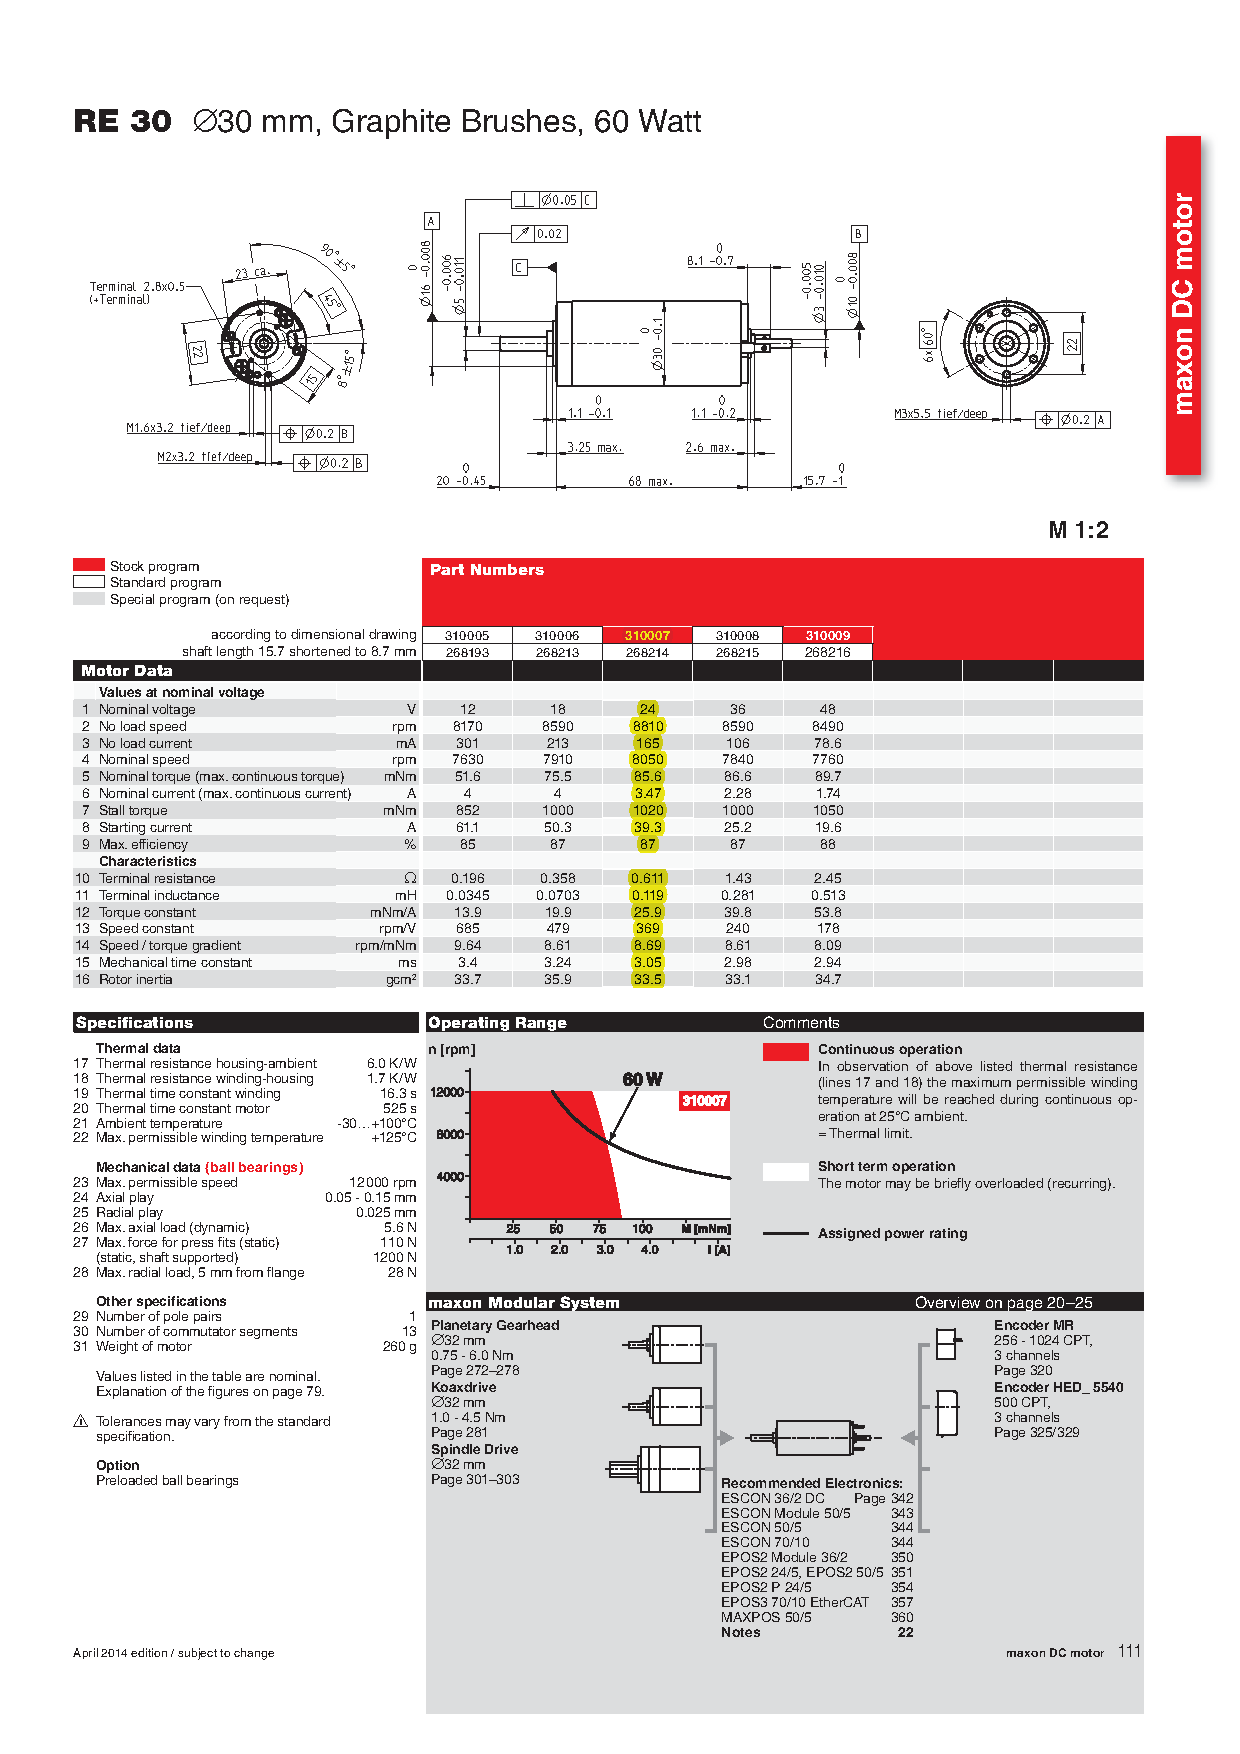
\includepdf[pages={1-},scale=0.8,pagecommand={}]{RE30.pdf}

La opción con \texttt{includegraphics} permite referirse a una página concreta y poner pies de figura.  Por ejemplo, en la figura~\ref{fig:hoja-datos} se muestra la hoja de especificaciones del motor empleado.

\begin{figure}[!ht]
\centering
\fbox{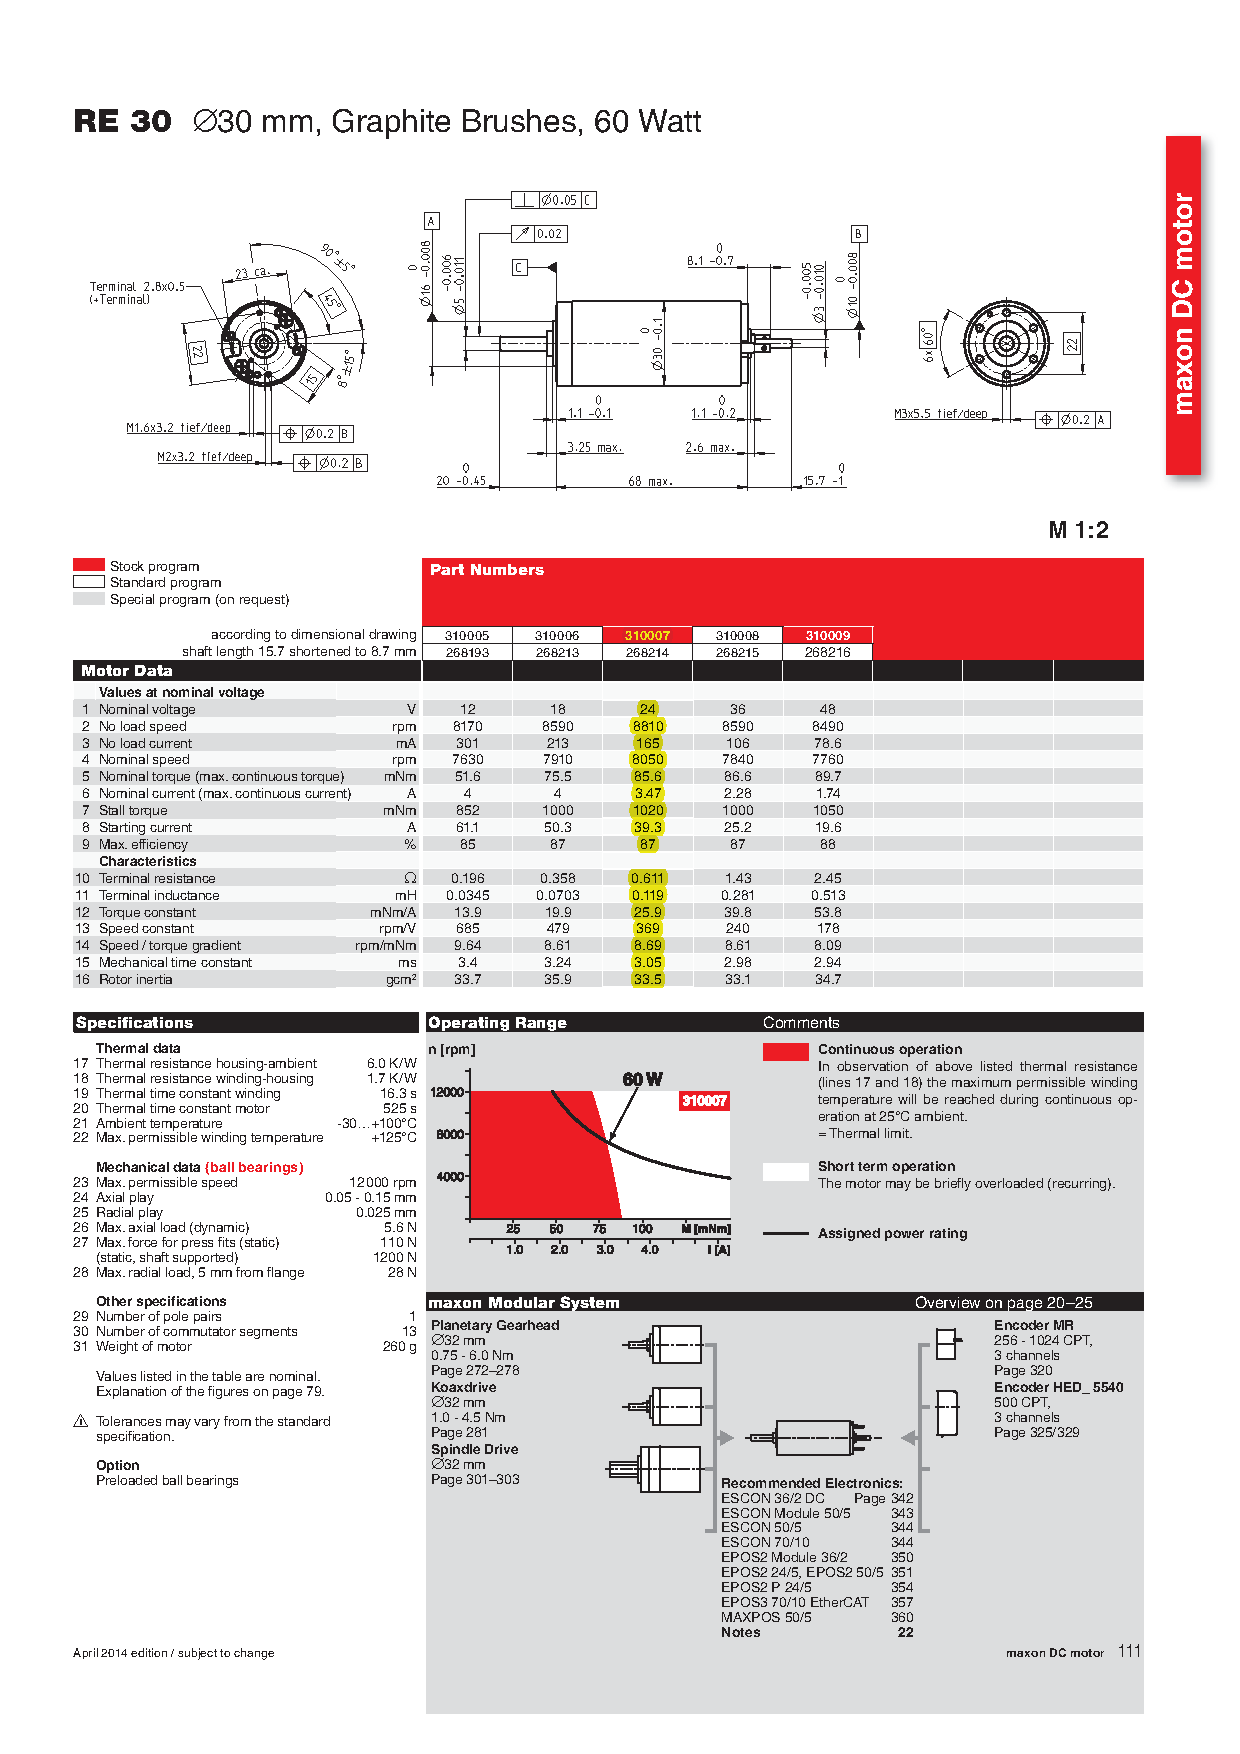
\includegraphics[page=1,width=.95\textwidth]{RE30.pdf}}
\caption{Figura ejemplo. Tomada de hoja de catálogo de \href{https://datasheets.globalspec.com/ds/17/MaxonPrecisionMotors/F1B48EDA-7358-46E6-964A-97E3BC5D921A}{motores DC con escobillas de grafito de Maxon} \copyright~2014 Maxon Motors. Reproducida con permiso.}
\label{fig:hoja-datos}
\end{figure}
	
\section{Código fuente} 
\label{sec:codigo-fuente}

Esto es un ejemplo de anexo. En este anexo se muestran algunos ejemplos de como plasmar código fuente.

Una opción es usar el paquete \texttt{lstlistings}.  Permite incluir archivos o parte de archivos directamente del proyecto con la orden \texttt{lstinputlisting}.

\lstinputlisting[language=Matlab,
    caption={Ejercicio 20 como texto incorporado},
    label=src:ej20-input
]{tex/latex/ejercicio20.m}

O bien se puede copiar el texto del programa o fragmento en un entorno \texttt{lstlisting} con las mismas opciones que la orden \texttt{lstinputlisting}.

\begin{lstlisting}[language=Matlab,
    caption={Ejercicio 20 como texto en línea.},
    label=src:ej20-online
]
function [T]=Ejercicio20(f,c)

T = char('B'*ones(8,8));

for i=1:8
    for j=1:8
        if ( (i==f) || (j==c) || (i+j==f+c) || (i-j==f-c) )
            T(i,j)='*';
        elseif ( rem(i+j,2)~=0 )
            T(i,j)='N';
        end
    end
end

T(f,c)='R';
\end{lstlisting}

\info{Te recomendamos que incluyas los archivos o parte de los archivos directamente del código de tu proyecto, ya sea mediante \texttt{lstinputlisting} o mediante \texttt{inputminted}.  De esta forma mantendrás sincronizado el documento con el código fuente.}

\noindent El paquete \texttt{lstlisting} te permite quitar los números y el marco, cuando el código se incluye como parte del texto. 

\begin{lstlisting}[language=Matlab,
    frame=none,numbers=none
]
function [T]=Ejercicio20(f,c)

T = char('B'*ones(8,8));

for i=1:8
    for j=1:8
        if ( (i==f) || (j==c) || (i+j==f+c) || (i-j==f-c) )
            T(i,j)='*';
        elseif ( rem(i+j,2)~=0 )
            T(i,j)='N';
        end
    end
end

T(f,c)='R';
\end{lstlisting}

\noindent Otra forma de incluir código es mediante el entorno \texttt{verbatim}.  Este método no tiene resalte de sintaxis ni facilidades de ningún tipo para definir etiquetas o numerar las líneas. 

\begin{verbatim}
function [T]=Ejercicio20(f,c)

T = char('B'*ones(8,8));

for i=1:8
  for j=1:8
    if ( (i==f) || (j==c) || (i+j==f+c) || (i-j==f-c) )
      T(i,j)='*';
    elseif ( rem(i+j,2)~=0 )
      T(i,j)='N';
    end
  end
end

T(f,c)='R';
\end{verbatim}

\noindent Otra forma alternativa a \texttt{lstlisting} es el paquete \texttt{minted}, que colorea el programa según el lenguaje empleado.

\setminted[matlab]{
    xleftmargin=20pt,
    linenos,
    breaklines,
    bgcolor=gris85}

\begin{minted}{matlab}
function [T]=Ejercicio20(f,c)

T = char('B'*ones(8,8));

for i=1:8
    for j=1:8
        if ( (i==f) || (j==c) || (i+j==f+c) || (i-j==f-c) )
            T(i,j)='*';
        elseif ( rem(i+j,2)~=0 )
            T(i,j)='N';
        end
    end
end

T(f,c)='R';
\end{minted}

\noindent O bien, usando la orden \texttt{inputminted} para incluir directamente un archivo Matlab.

\inputminted{matlab}{tex/latex/ejercicio20.m}

}

% La bibliografía no suele ir numerada porque se pone después de los anexos.
% No se debe poner antes de los anexos porque si se cita una referencia en
% un anexo sería una backward reference, que deben evitarse a toda costa
\cleardoublepage
\hypertarget{ch:bibliografia}{%
    \printbibliography[heading=bibintoc,title={Bibliografía}]}
\cleardoublepage

\end{document}
